\documentclass[a4paper]{article}

\usepackage{pgfplots}

\pgfplotsset{compat=1.8}


\begin{document}

%\tracingcommands=2\tracingmacros=2
\fbox{%
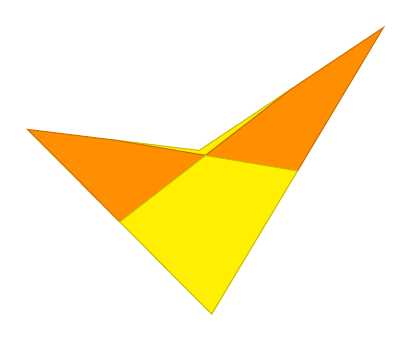
\begin{tikzpicture}
    \begin{axis}[
		xmin=-10,xmax=10,
		zmin=-50,
		hide axis, %clip=false,
	]
	\addplot3[surf,samples=3] {x*y};
	\end{axis}
\end{tikzpicture}%
}


 \fbox{%
  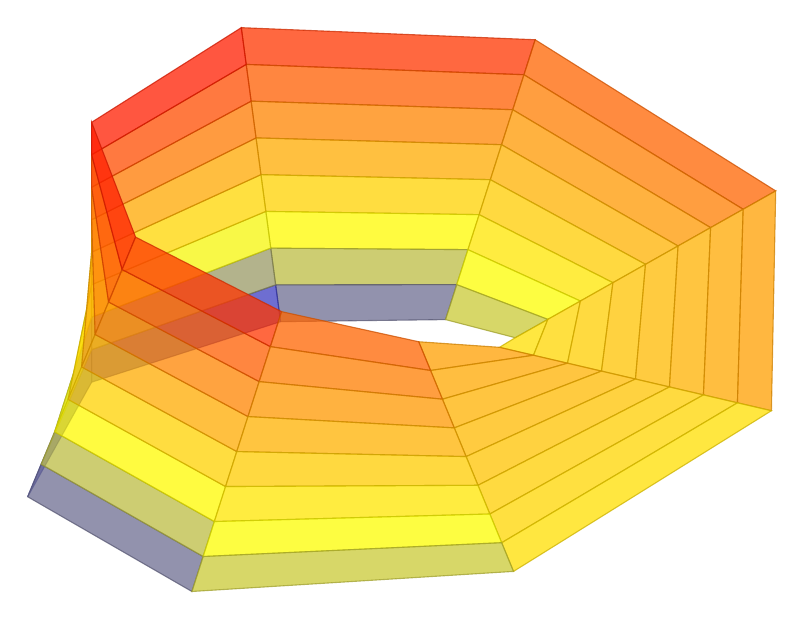
\begin{tikzpicture}
    \begin{axis}[
		axis equal,
		scale=2,
		axis lines=none, %clip=false,
	]
      \addplot3[surf,samples=9,domain=-1:1,y domain=0:2*pi,z buffer=sort,opacity=0.75]
         ({cos(deg(y)) * (1 + x/2 * cos(deg(y)/2))},
         {sin(deg(y)) * (1 + x/2 * cos(deg(y)/2))},
         {x/2 * sin(deg(y)/2)});
    \end{axis}
  \end{tikzpicture}}


\end{document}

